\documentclass[11pt,a4paper]{article}

%
% $Id: userguide.tex 526 2007-10-31 08:57:09Z schnelle $
%

\usepackage[latin1]{inputenc}
\usepackage{graphics}
\usepackage{graphicx}
\usepackage{url}
\usepackage{listings}
\usepackage{xcolor}
\usepackage{jvoicexml}

\title{JVoiceXML Vendor Guide}
\version{0.1}
\author{Dr. Dirk Schnelle-Walka}
\email{dirk.schnelle@jvoicexml.org}
\date{\today}

\begin{document}
\pagestyle{empty}
\lstset{language=Java,language=XML,
        backgroundcolor=\color{lightgray},
        basicstyle=\small,
        numbers=left,
        numberstyle=\tiny,
        stepnumber=5}

\maketitle

\pagestyle{headings}

\tableofcontents

\newpage

\begin{abstract}
This documents describes the API of JVoiceXML from the vendor's point of
view. It provides information about how to hook your custom implementation
platform into the JVoiceXML voice browser.
\end{abstract}


\section{Introduction}
\label{sec:introduction}

JVoiceXML is a free VoiceXML~\cite{w3.org:voicexml} implementation written in 
the JAVA programming language. It offers a library for easy VoiceXML
document creation and a VoiceXML interpreter to process 
VoiceXML documents using JAVA standard APIs such as JSAPI~\cite{sun:jsapi} and
JTAPI~\cite{sun:jsapi}.

VoiceXML is hosted at SourceForge~\cite{sourceforge} as an open source project.
You find everything that is related to this project under
\url{http://sourceforge.net/projects/jvoicexml/}.
The work on the browser is still in progress and not all tags are
supported. You are invited to help us finishing the work to make this
project a success.

This document provides information on how to hook your custom implemenation
paltform into the JVoiceXML voice browser. It is assumed that readers are
familiar with the concepts of VoiceXML and Java programming.

This document refers to UNIX and Windows systems. JVoiceXML will work with 
any other operating systems that support Java 5, too.

Nobody is perfect, so you may find some errors or small things to correct.
Please let me know if you think you found something that should be written
differently or should be added.

\section{Architectural Overview}
\label{sec:arch-overv}

Before going into detail the general architecture and concepts are presented.
The basic architecture is shown in figure~\ref{fig:main-components}.
\begin{figure}
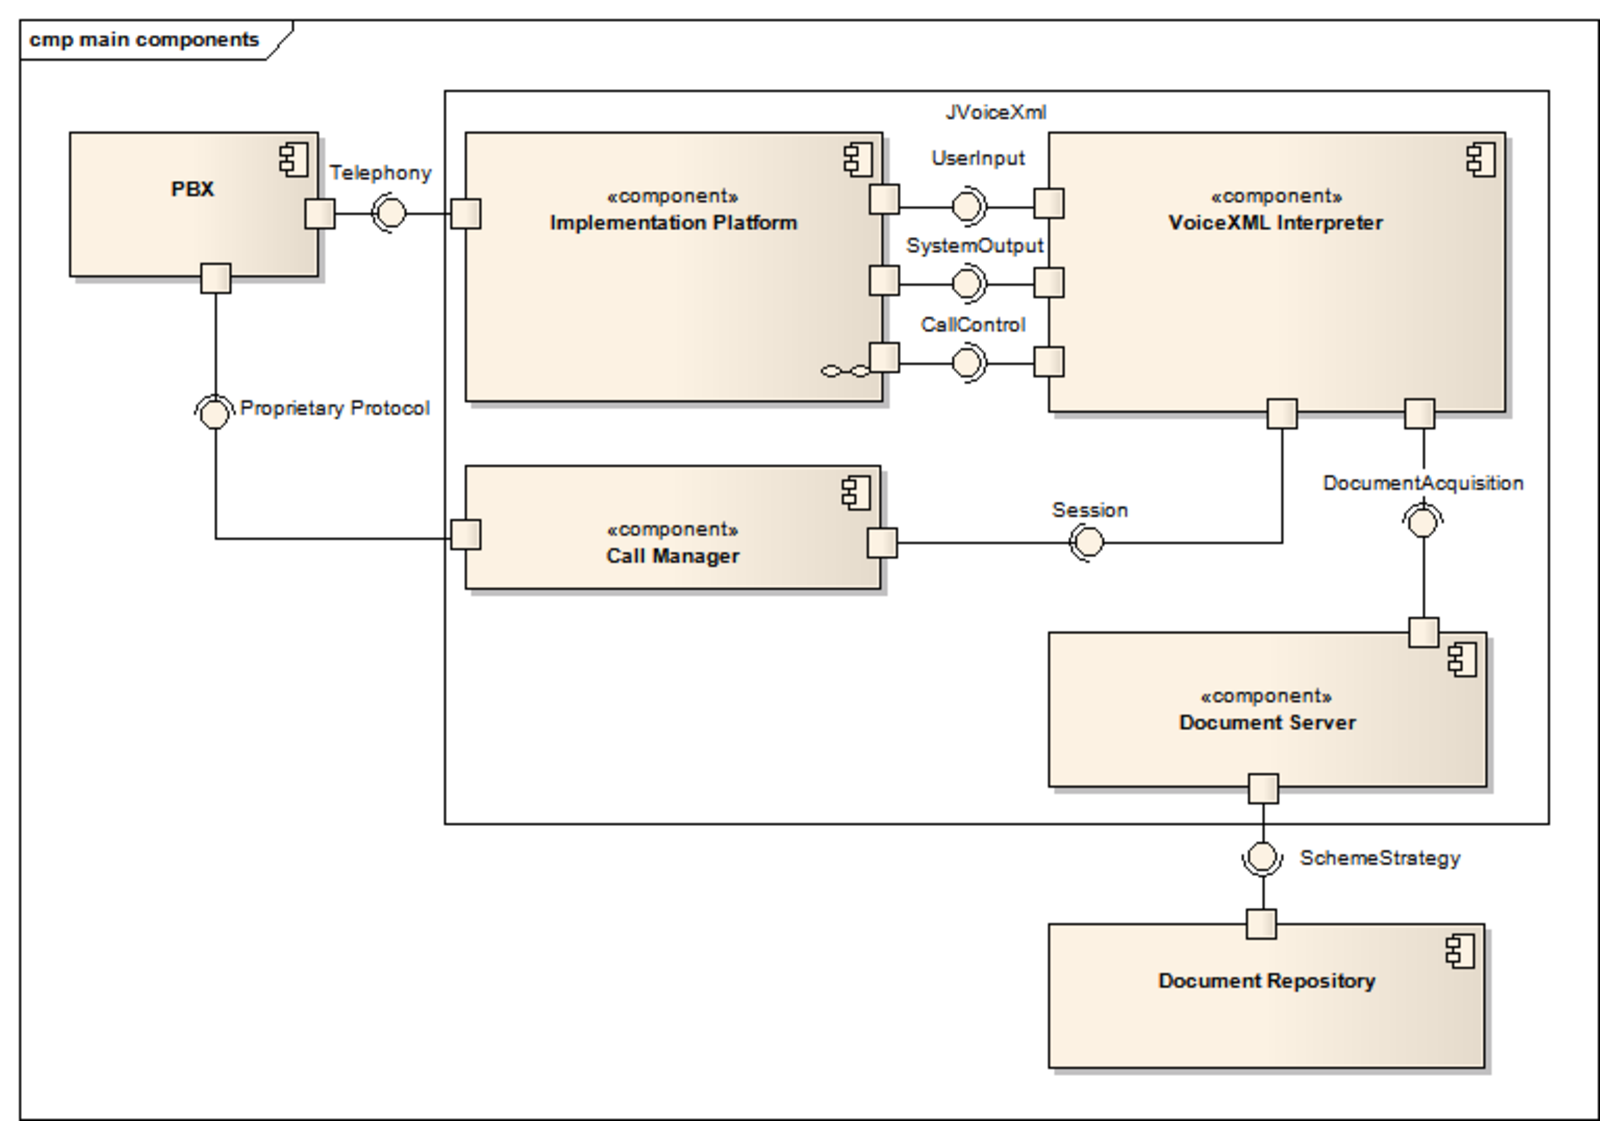
\includegraphics[width=\linewidth]{cd-main-components}
\caption{Basic architecture of JVoiceXML}
\label{fig:main-components}
\end{figure}
The point of interest is the \emph{Implemtation Platform}.
Figure~\ref{fig:implementationplatform} shows the composite parts of that
component.
\begin{figure}
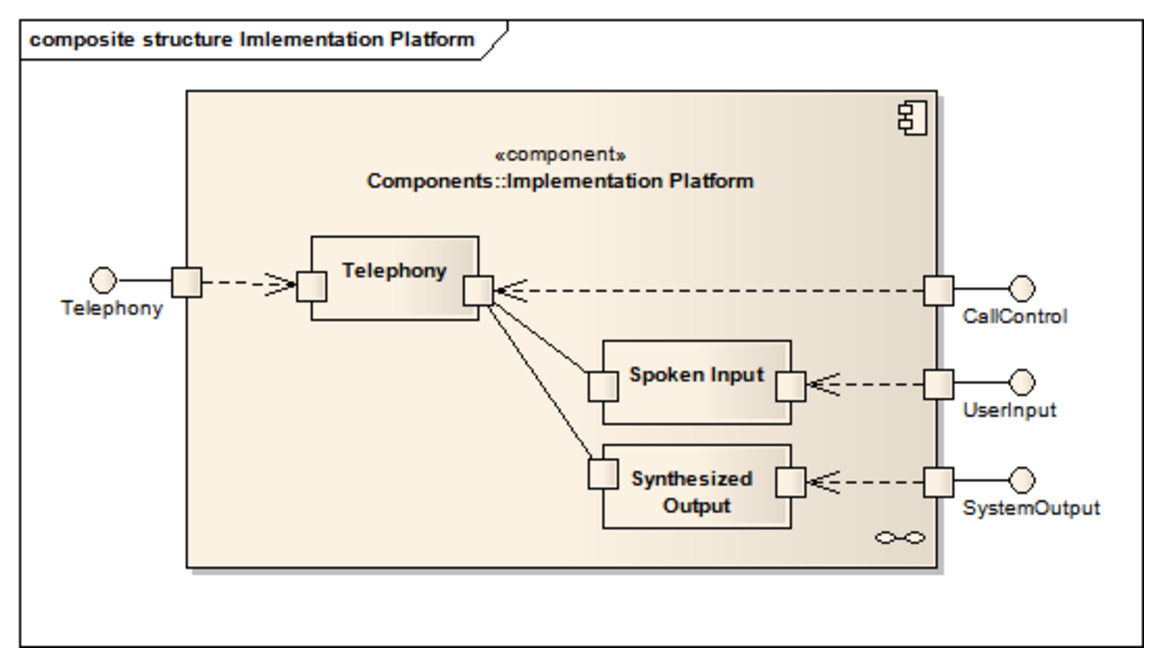
\includegraphics[width=\linewidth]{csd-implementation-platform}
\caption{Compositite parts of the implementation platform}
\label{fig:implementationplatform}
\end{figure}

\section{Steps to your own implementation platform}

\subsection{RemoteClient}

A remote client is a data container that holds all the information that is
needed to connect the server side resources. Therefore you have to implement
the \lstinline[language=Java]{org.jvoicexml.RemoteClient} interface. This
container should hold all the information that is needed to connect to your
client application from the JVoiceXML resources.

The identification is based on strings. Choose a unique name for each of your
resource types. It is legal to have the same name for all your types.

This class must also implement \lstinline[language=Java]{java.io.Serializabe}
to stream the object from your client to the JVoiceXML voice browser.

\subsection{Resources}

The first step is to write your own implementations of the resources:
\begin{itemize}
  \item \lstinline[language=Java]{org.jvoicexml.implementation.SpokenInput}
  \item
  \lstinline[language=Java]{org.jvoicexml.implementation.SynthesizedOutput}
  \item \lstinline[language=Java]{org.jvoicexml.implementation.Telephony}
\end{itemize}

Your \lstinline[language=Java]{SynthesizedOutput} implementation should maintain
a queue of speakables that should be sent to your client.

Your \lstinline[language=Java]{Telephony} implementation should be able to
conect to your client. It takes the speakables from your Your
\lstinline[language=Java]{SynthesizedOutput} Sending it to your client and also
retrieve inputs from the client. These are forwarded to your 
\lstinline[language=Java]{SpokenInput} implementation. The latter one is
responsible to notify the JVoiceXML voice browser about incoming speech events.

 
The resources communicate with
the JVoiceXML voice browser using a notification mechanism. Hence it is important that the custom resource classes also
implement the corresponding notification interfaces.

\begin{itemize}
  \item the \lstinline[language=Java]{SpokenInput} resource must also implement
  \\
  \lstinline[language=Java]{org.jvoicexml.implementation.ObservableSpokenInput}
  \item the \lstinline[language=Java]{SynthesizedOutput} resource must also
  implement \\
  \lstinline[language=Java]{org.jvoicexml.implementation.ObservableSynthesizedOutput}
  \item the \lstinline[language=Java]{Telephony} resource must also implement \\
  \lstinline[language=Java]{org.jvoicexml.implementation.ObservableTelephony}
\end{itemize}

\subsection{Resource factories}

The implementation platform retrieves the resources via a
\lstinline[language=Java]{org.jvoicexml.implementation.ResourceFactory}.
Implement a factory for each of your resources.

Return the type that you defined in your
\lstinline[language=Java]{RemoteClient} implementation.

\subsection{JVoiceXML configuration}

JVoiceXML retrieves the resource factories via dependency injection from
\lstinline{$JVOICEXML_HOME/config/implementation.xml}.

Add your resource factories to the configuration as shown in the following
example:

\begin{lstlisting}[language=XML]
<bean id="implementationplatform"
 class="\ldotsJVoiceXmlImplementationPlatformFactory">
  <property name="synthesizedoutput">
   <list>
    <bean class="yourpackage.YourSynthesizedOutputFactory">
   </list>
  </property>
  <property name="spokeninput">
   <list>
    <bean class="yourpackage.YourSpokenInputFactory">
   </list>
  </property>
  <property name="telephony">
   <list>
    <bean class="yourpackage.YourTelephonyFactory">
   </list>
  </property>
</bean>
\end{lstlisting}

\subsection{CLASSPATH adaption}

When you are done, add your classes to the \lstinline{CLASSPATH} and start the
JVoiceXML voice browser.

\bibliography{vendorguide}
\bibliographystyle{plain}

\end{document}
